\documentclass[14pt,aspectratio=169]{beamer}

\usepackage[T1]{fontenc}
\usepackage[utf8]{inputenc}
\usepackage{lmodern}

\usepackage{gensymb}


\usetheme{Warsaw}
\usecolortheme{albatross}

\setbeamertemplate{footline}[frame number]
\setbeamercovered{transparent}


\title[MSLP]{Mean Sea Level Pressure}

\author{Johan Montelius}
\date{2026-06-03}

\begin{document}

\begin{frame}
\titlepage
\end{frame}
 
\begin{frame}{the data}

\vspace{20pt}\uncover<2->{What data do we have?}
  \vspace{20pt}

\begin{itemize}
  \item\uncover<3,7>{grided data of calculated mslp}
  \item\uncover<4,7>{$2.5\degree \times 2.5\degree$, $10512$ cells}
  \item\uncover<5,7>{mean montly values, 1978 - 2026}
  \item\uncover<6,7>{stations, baloons, satellite ... coverage?}
\end{itemize}

\end{frame}


\begin{frame}{Stockholm $lat 57.5\degree \; lon\; 17.5\degree$}

\begin{figure}
    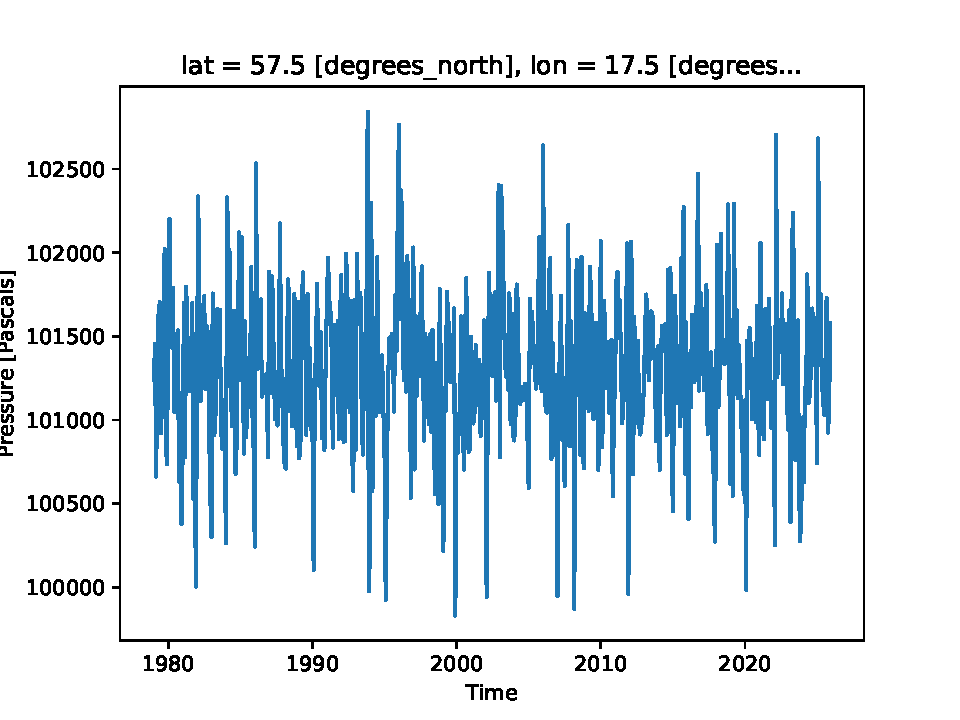
\includegraphics[width=0.4\textwidth]{stockholm-full.pdf}%
    \hfill
    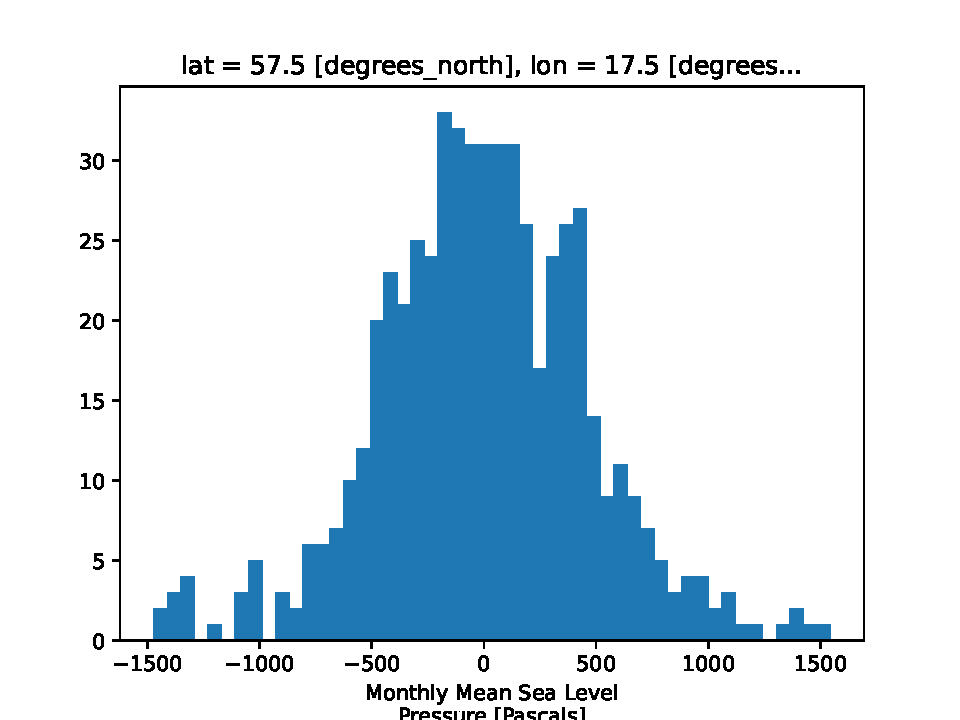
\includegraphics[width=0.4\textwidth]{stockholm-hist.pdf}
\end{figure}

\end{frame}


\begin{frame}{The globe mean pressure}

\begin{figure}
    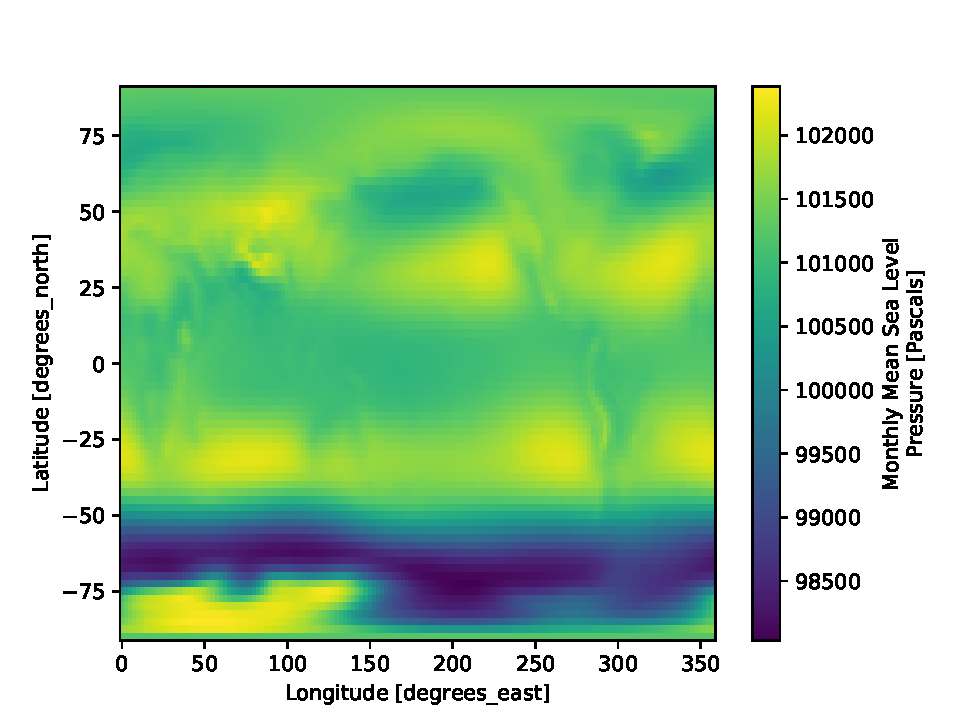
\includegraphics[width=0.4\textwidth]{mean-global.pdf}
\end{figure}


\end{frame}

\begin{frame}{The globe mean pressure}

\begin{figure}
    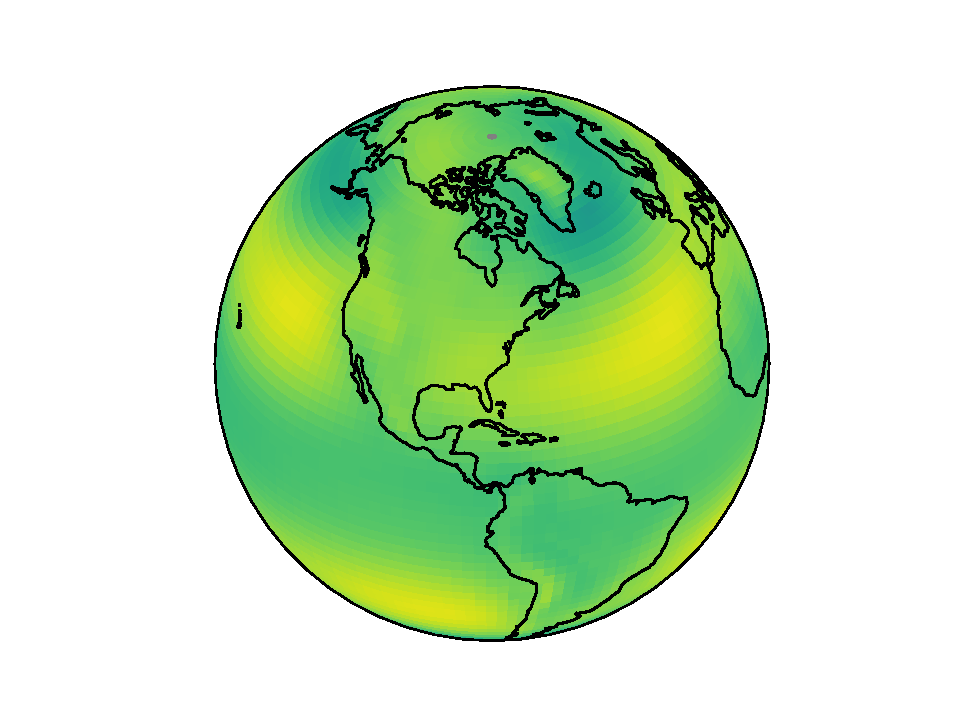
\includegraphics[width=0.4\textwidth]{mean-north.pdf}%
    \hfill
    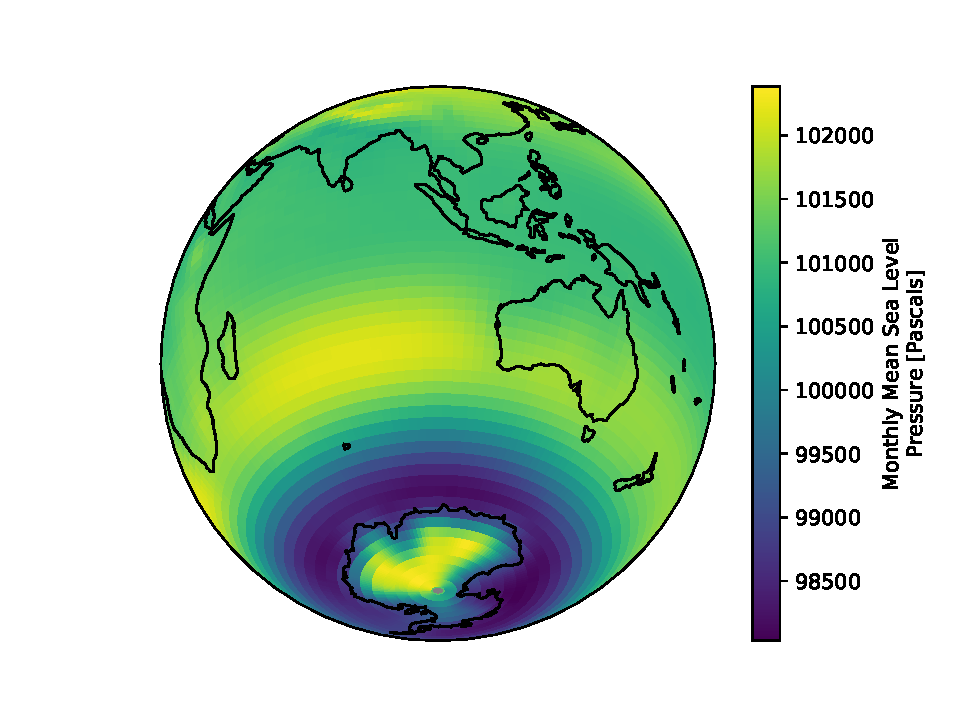
\includegraphics[width=0.4\textwidth]{mean-south.pdf}
\end{figure}

\end{frame}

\begin{frame}{Difference first/last period}

\begin{figure}
    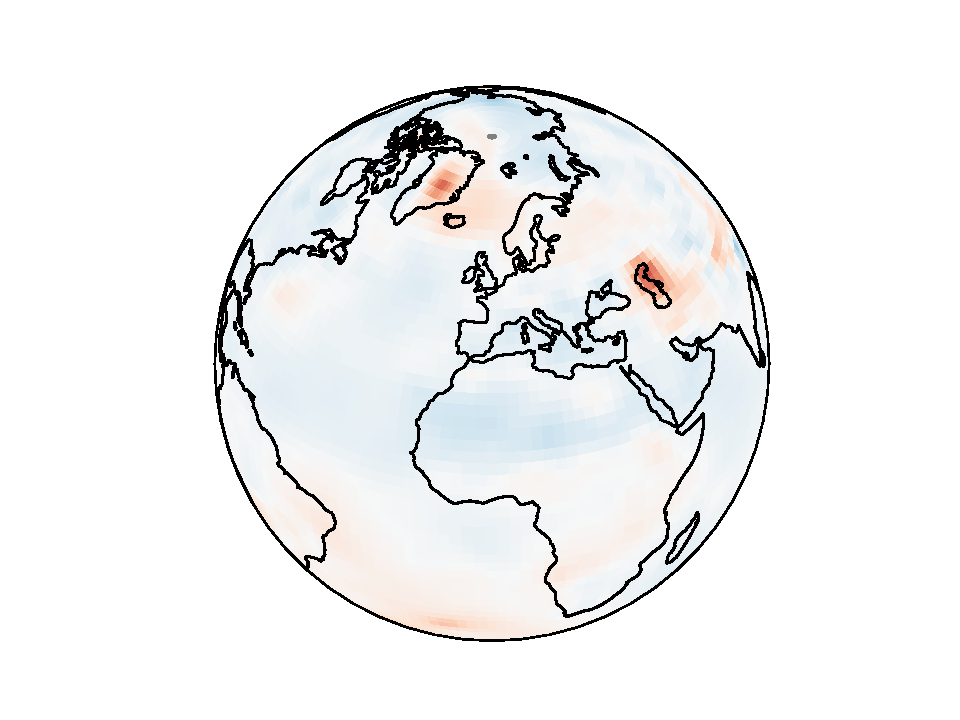
\includegraphics[width=0.4\textwidth]{dif-north.pdf}%
    \hfill
    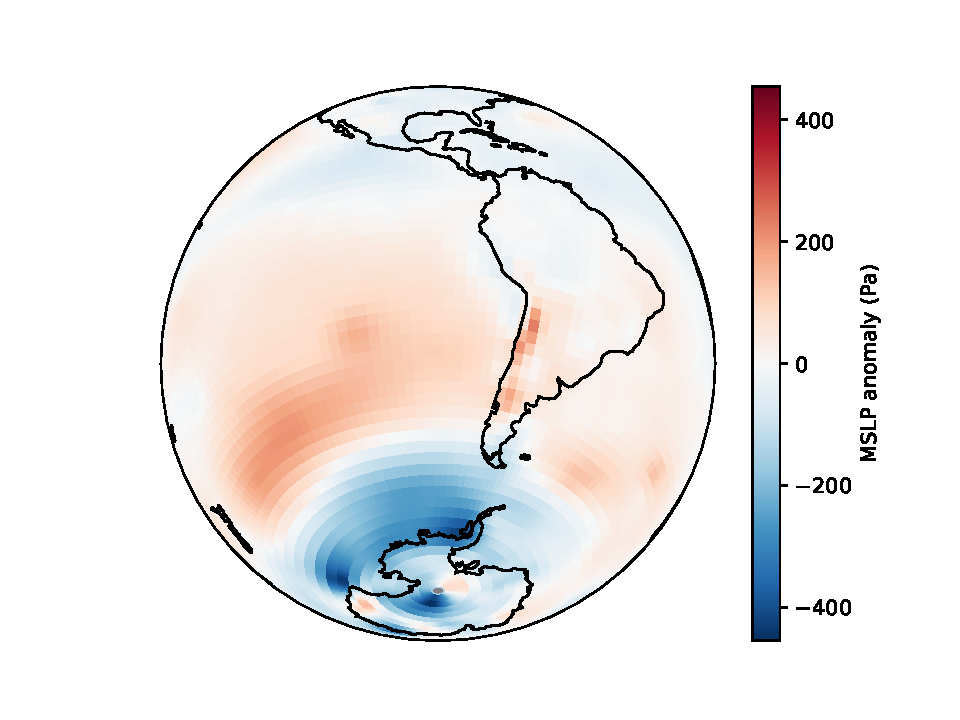
\includegraphics[width=0.4\textwidth]{dif-south.pdf}
\end{figure}

\end{frame}

\begin{frame}{Significant changes}

\begin{figure}
    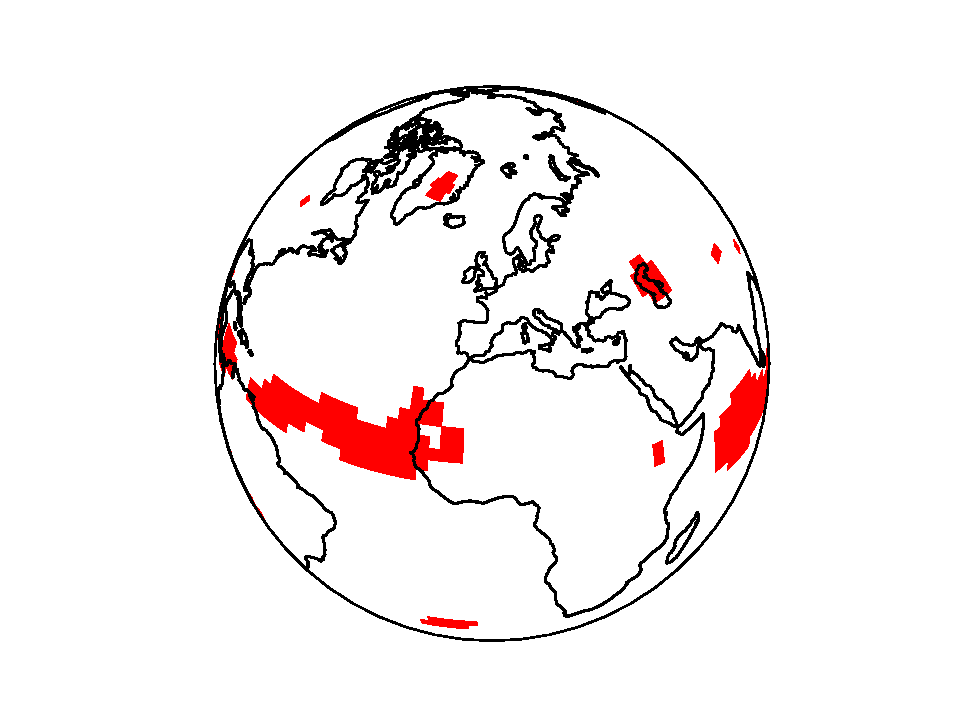
\includegraphics[width=0.4\textwidth]{sig-north.pdf}%
    \hfill
    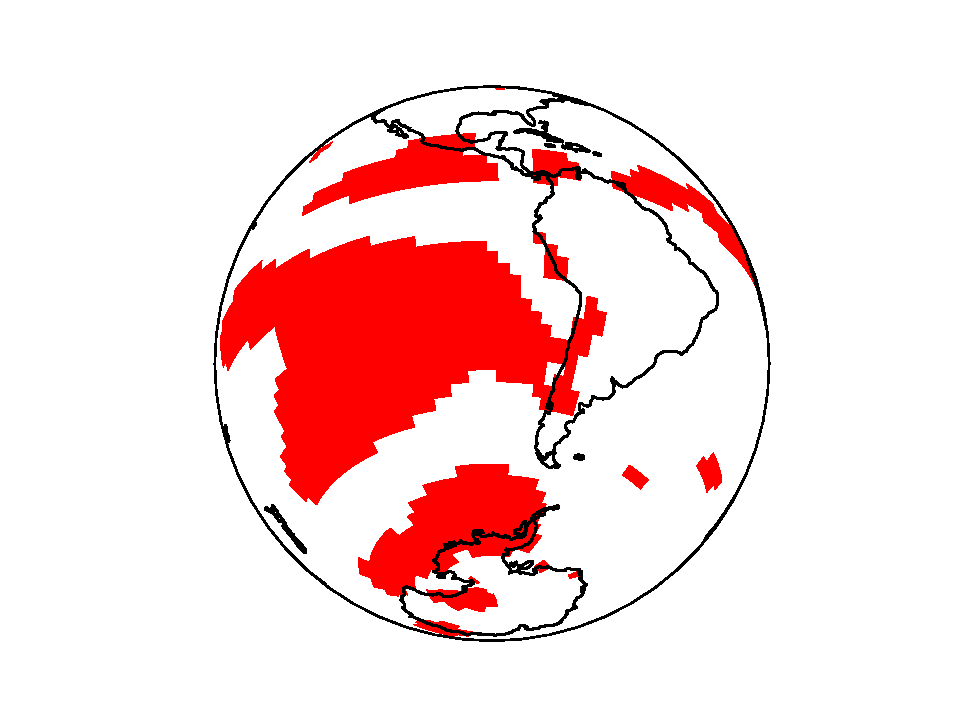
\includegraphics[width=0.4\textwidth]{sig-south.pdf}
\end{figure}

\end{frame}

\begin{frame}{changes during a year}

\begin{figure}
    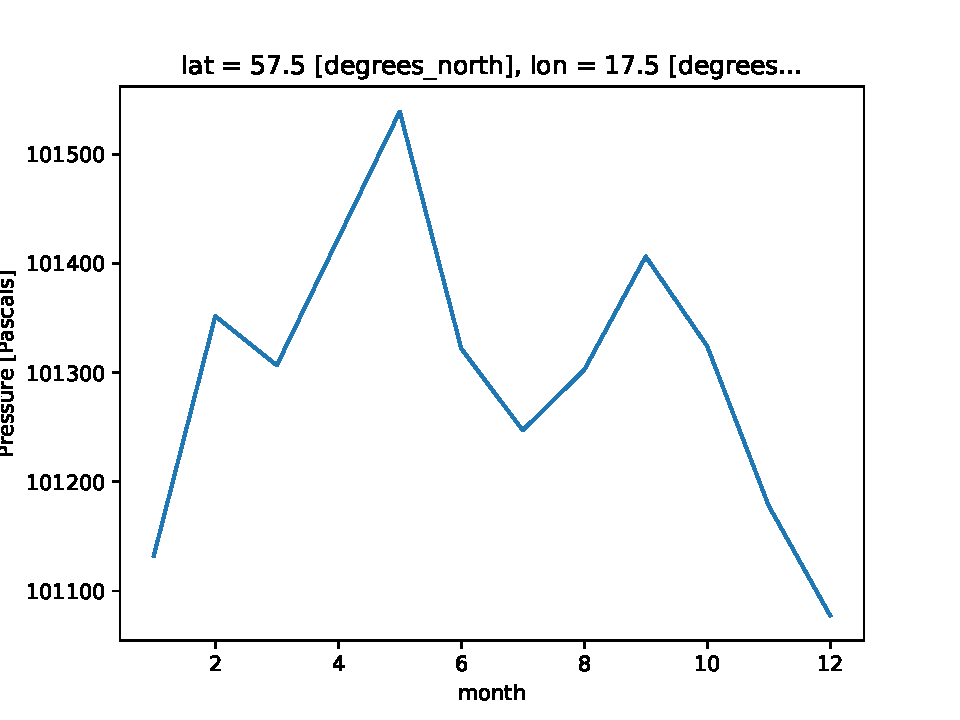
\includegraphics[width=0.4\textwidth]{stockholm-year.pdf}%
    \hfill
    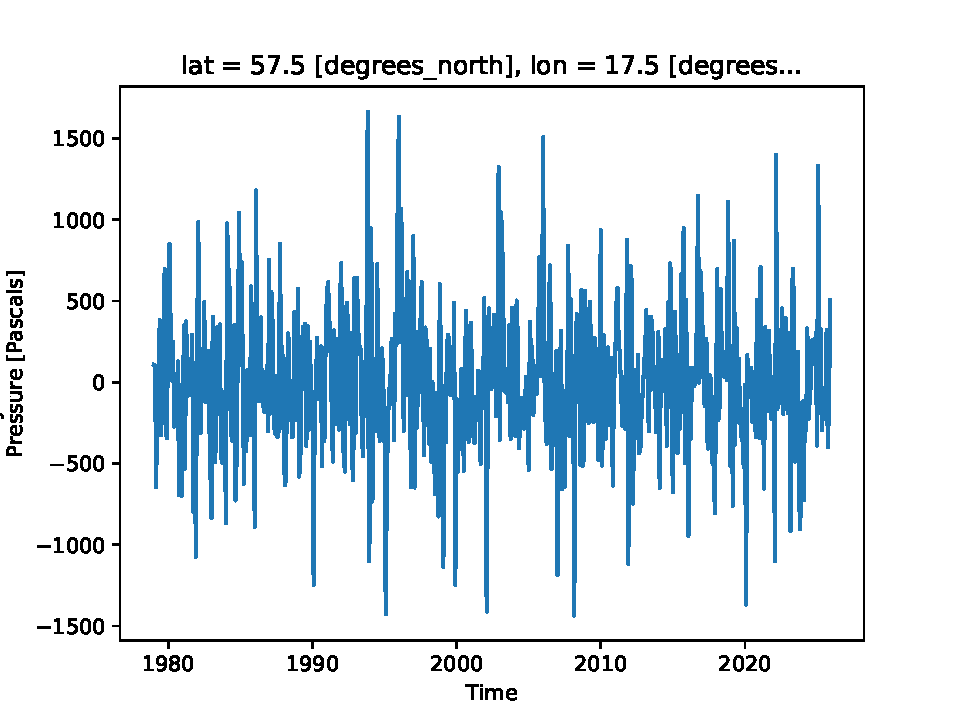
\includegraphics[width=0.4\textwidth]{stockholm-anom.pdf}
\end{figure}

\end{frame}

\begin{frame}{Winter (Dec,Jan,Feb) - EOF}

\begin{figure}
    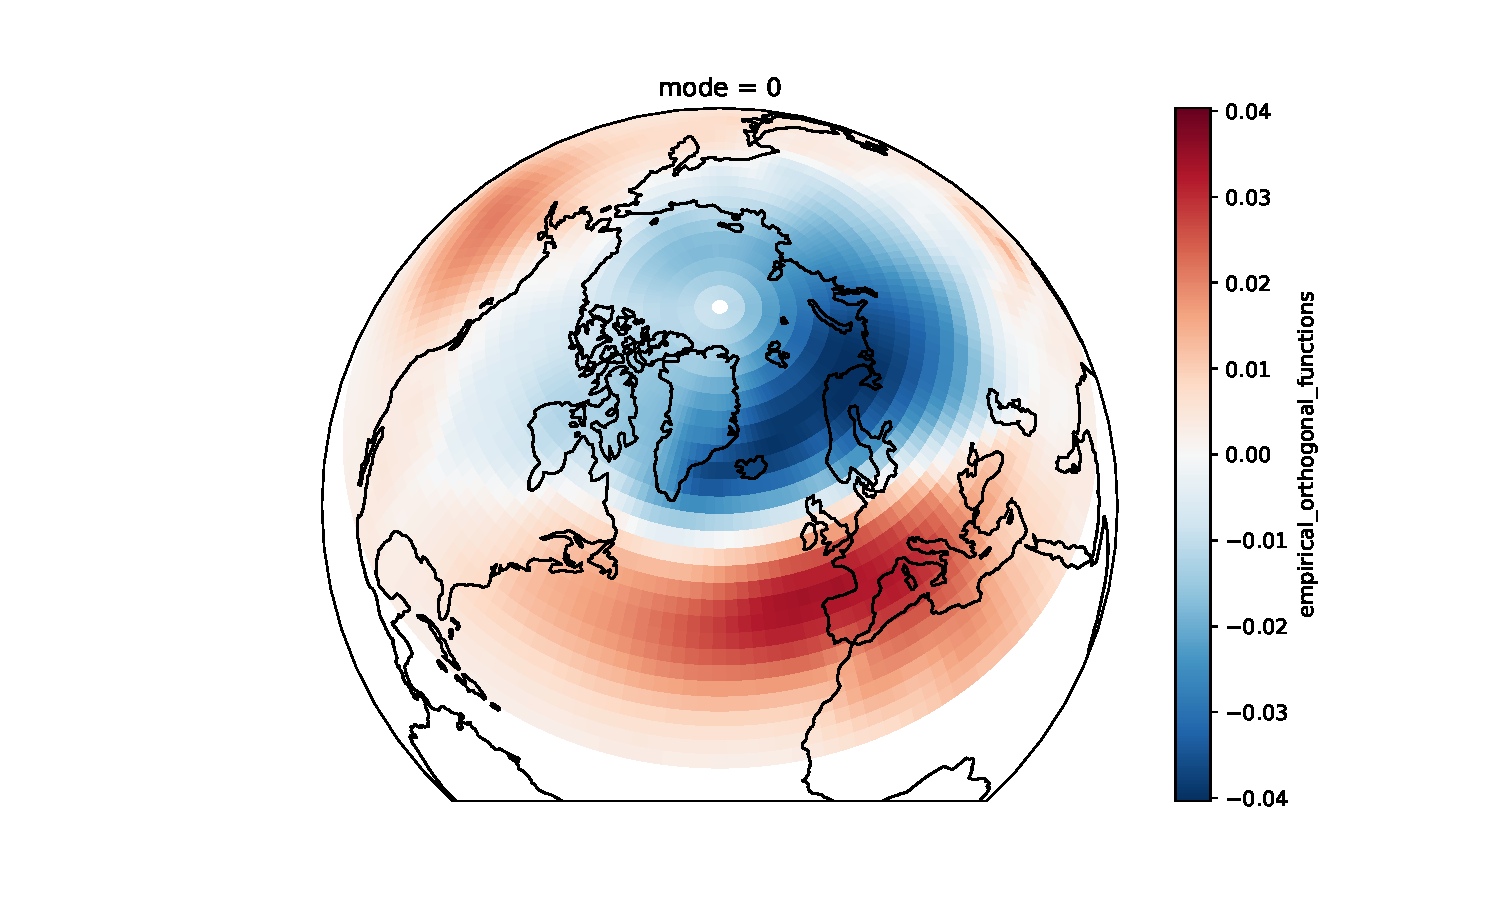
\includegraphics[width=0.4\textwidth]{winter-nh-eof.pdf}%
    \hfill
    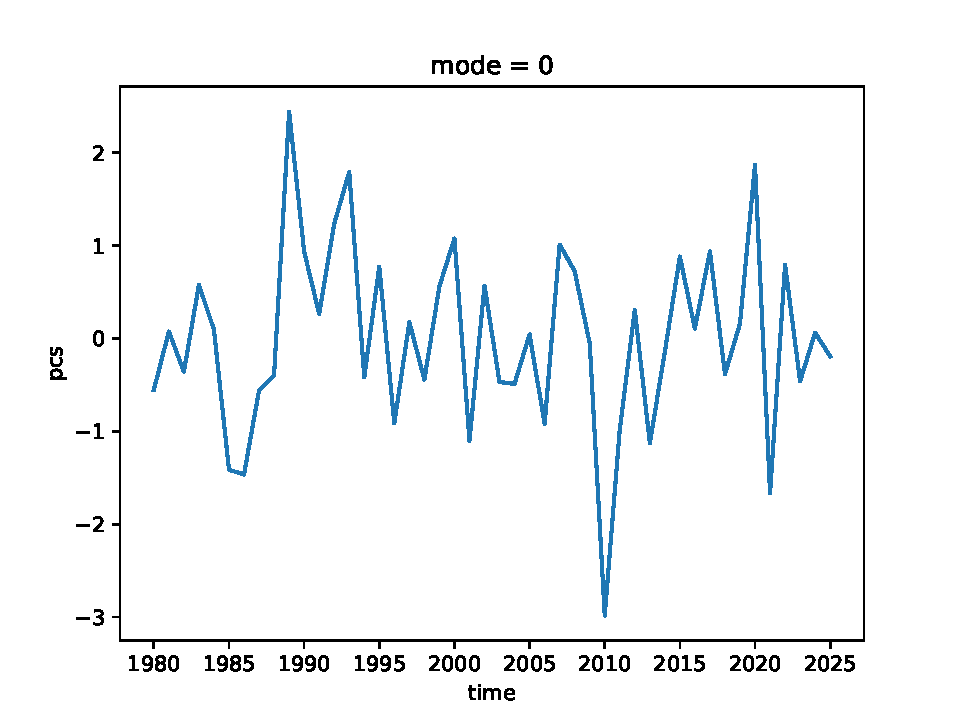
\includegraphics[width=0.4\textwidth]{winter-nh-pc1.pdf}
\end{figure}

\end{frame}

\begin{frame}{Winter /Dec, Jan, Feb) - Period of cycle - Fourier}

\begin{figure}
    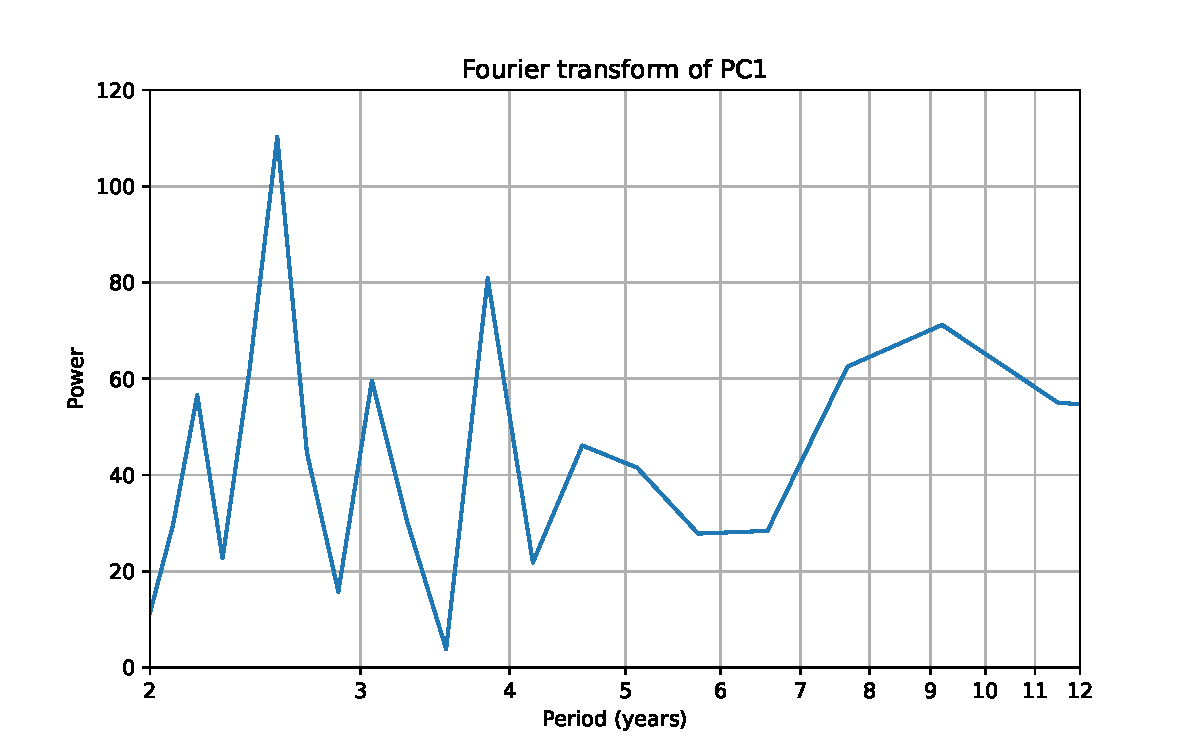
\includegraphics[width=0.4\textwidth]{pc1-fourier.pdf}%
    \hfill
    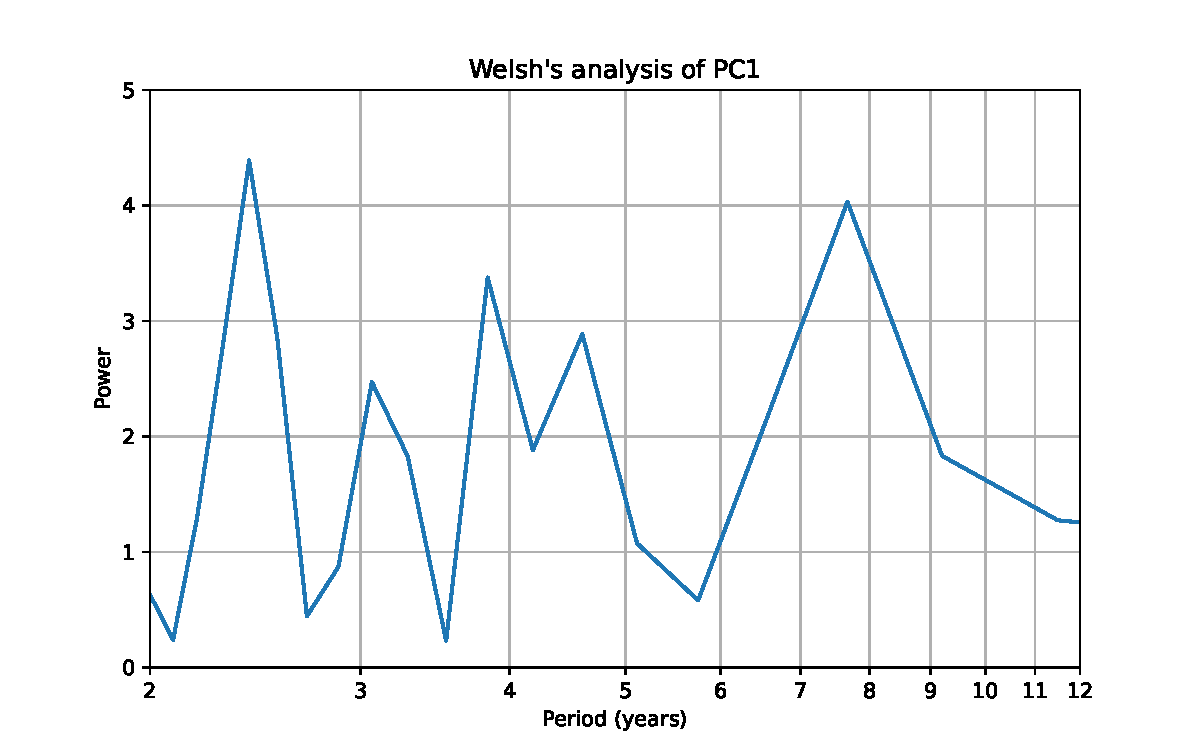
\includegraphics[width=0.4\textwidth]{pc1-welsh.pdf}
\end{figure}

\end{frame}


\begin{frame}{Darwin - Tahiti}

\begin{table}[ht!]
\centering
\begin{tabular}{ c c c }
 \textbf{EOF} & \textbf{ Darwin} & \textbf{ Tahiti} \\
\hline\\
EOF1 & -0.70 & 0.71\\
EOF2 & -0.71 & -0.70\\
\end{tabular}
\caption{EOF of Darwin vs Tahiti}
\label{tab:darwin-tahiti-eof}
\end{table}

\end{frame}

\begin{frame}{Darwin - Tahiti}

\begin{figure}
    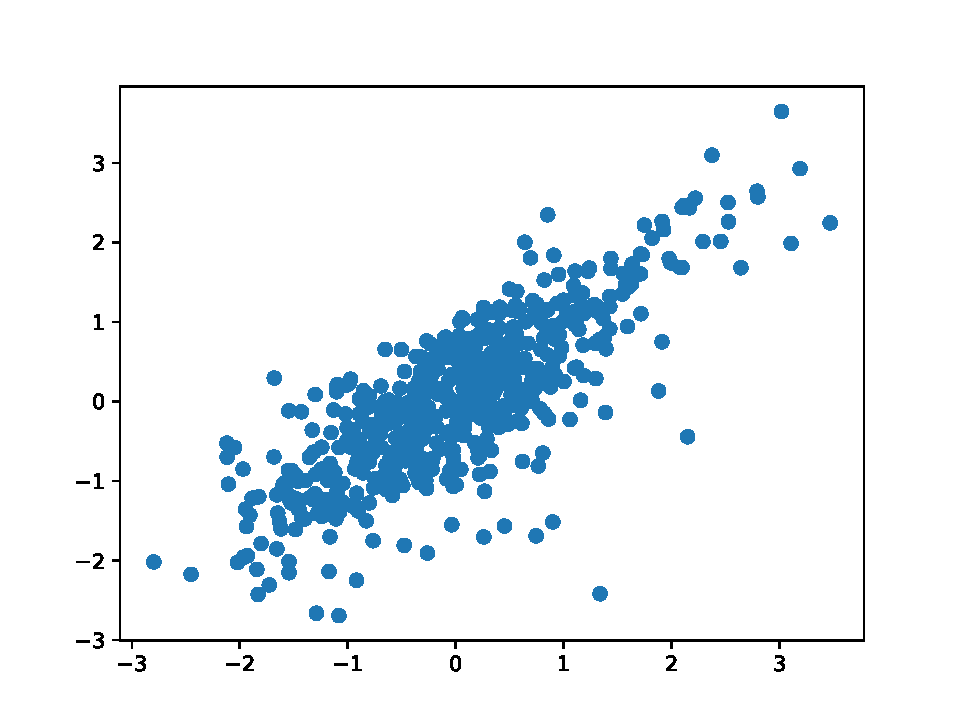
\includegraphics[width=0.4\textwidth]{darwin-tahiti-scatter.pdf}
\end{figure}


\end{frame}

\begin{frame}{Darwin - Tahiti}

\begin{figure}
    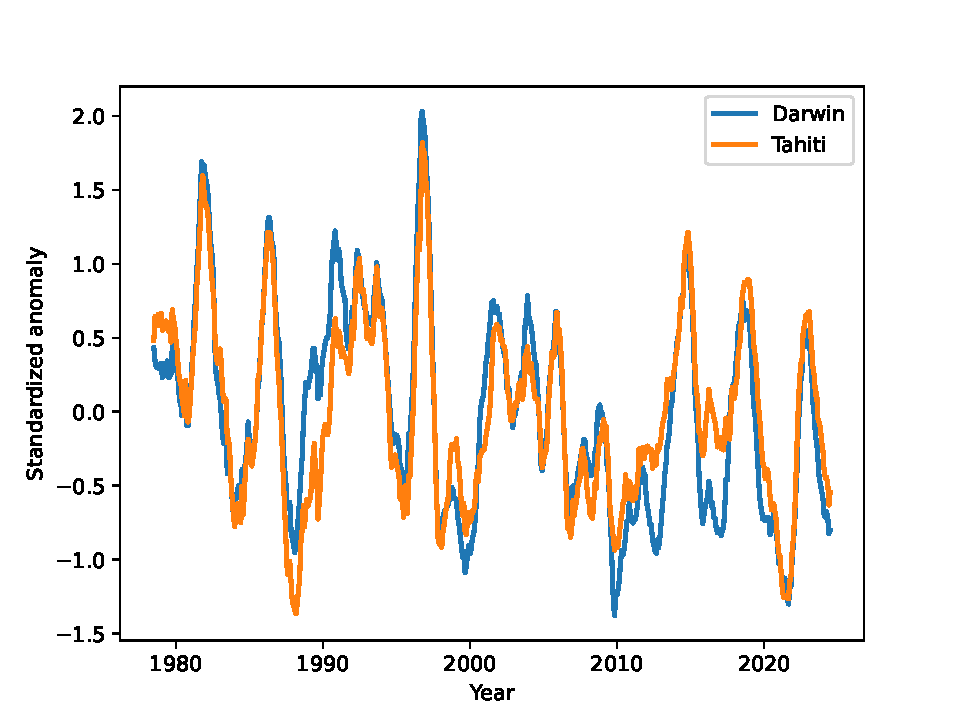
\includegraphics[width=0.4\textwidth]{darwin-tahiti-running.pdf}
\end{figure}


\end{frame}

\begin{frame}{Darwin - Tahiti  PC1 Fourier}

\begin{figure}
    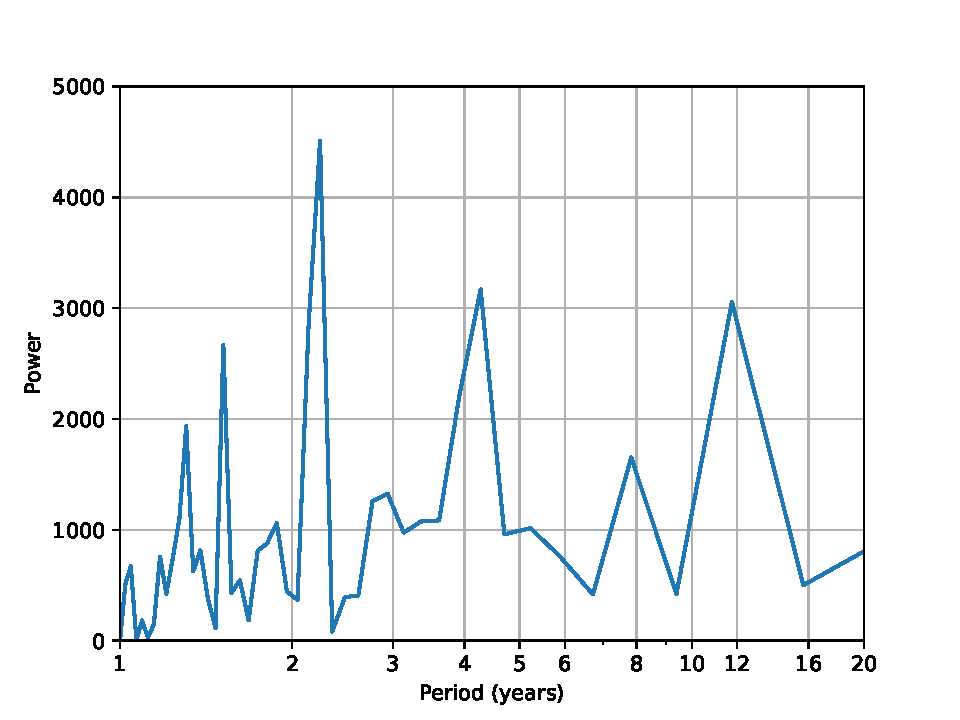
\includegraphics[width=0.4\textwidth]{darwin-tahiti-pc1.pdf}
\end{figure}

\end{frame}

\begin{frame}{Darwin/Tahiti - the Pacific}

\begin{figure}
    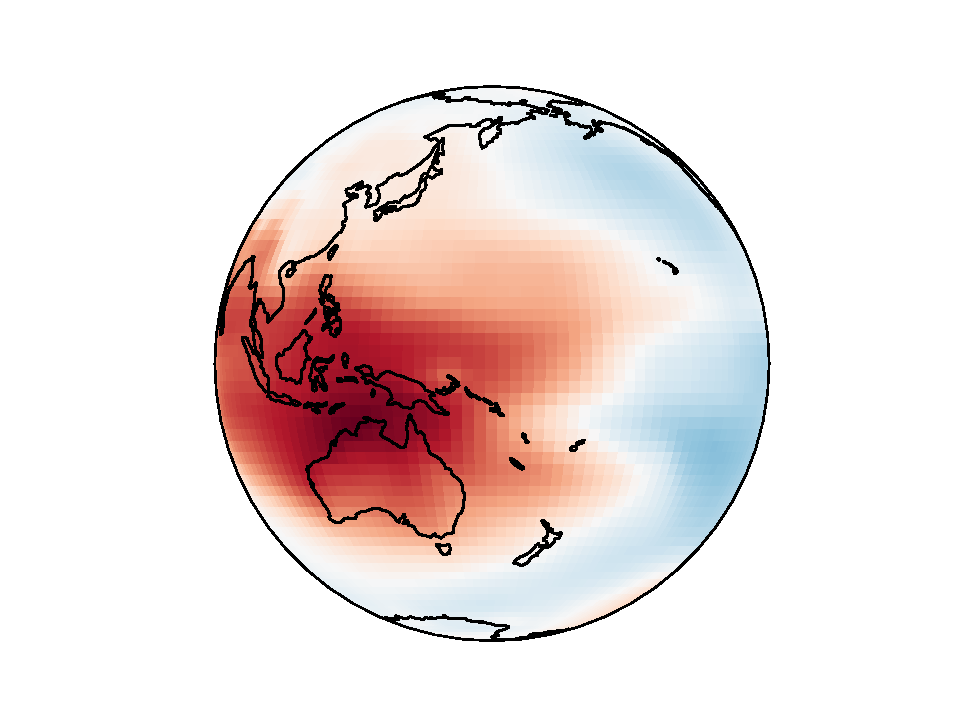
\includegraphics[width=0.4\textwidth]{darwin-pacific.pdf}%
    \hfill
    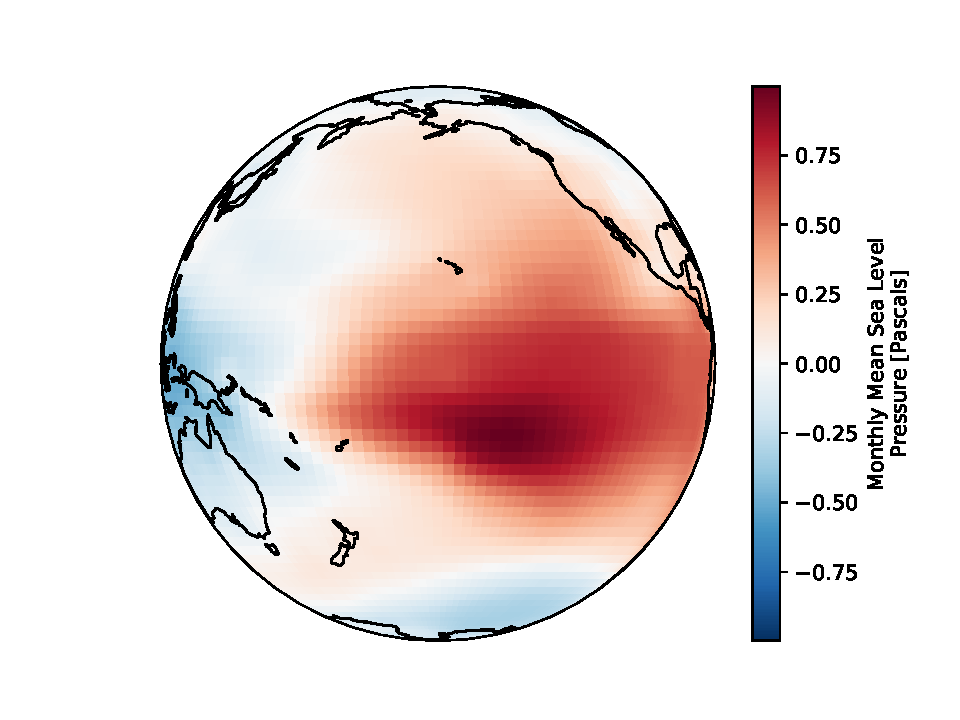
\includegraphics[width=0.4\textwidth]{tahiti-pacific.pdf}
\end{figure}


\end{frame}

\begin{frame}{Darwin/Tahiti - Europe}

\begin{figure}
    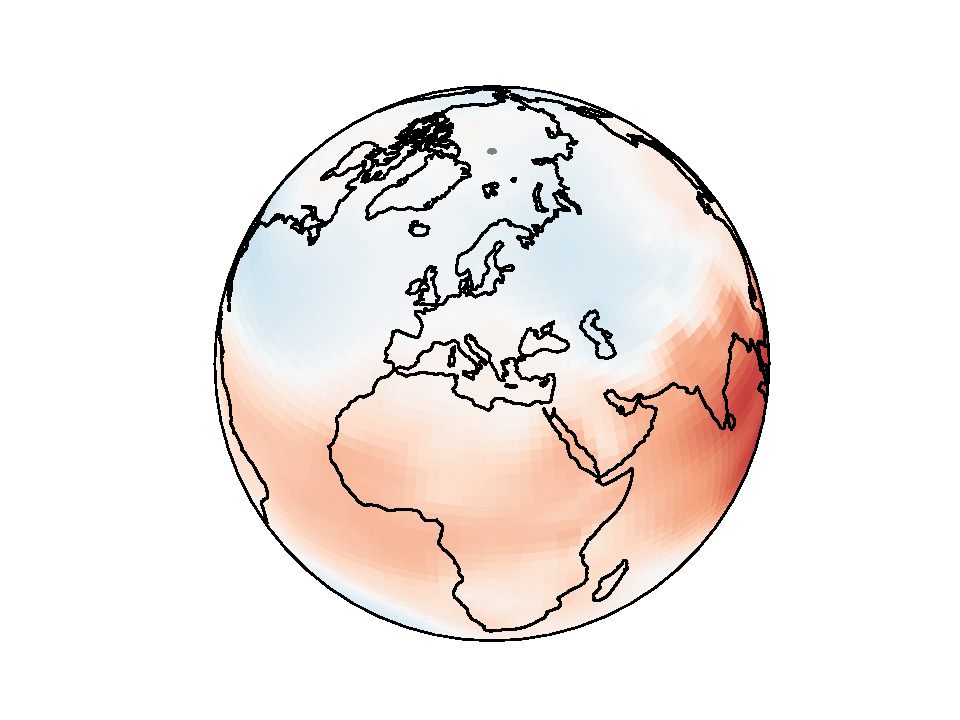
\includegraphics[width=0.4\textwidth]{darwin-europe.pdf}%
    \hfill
    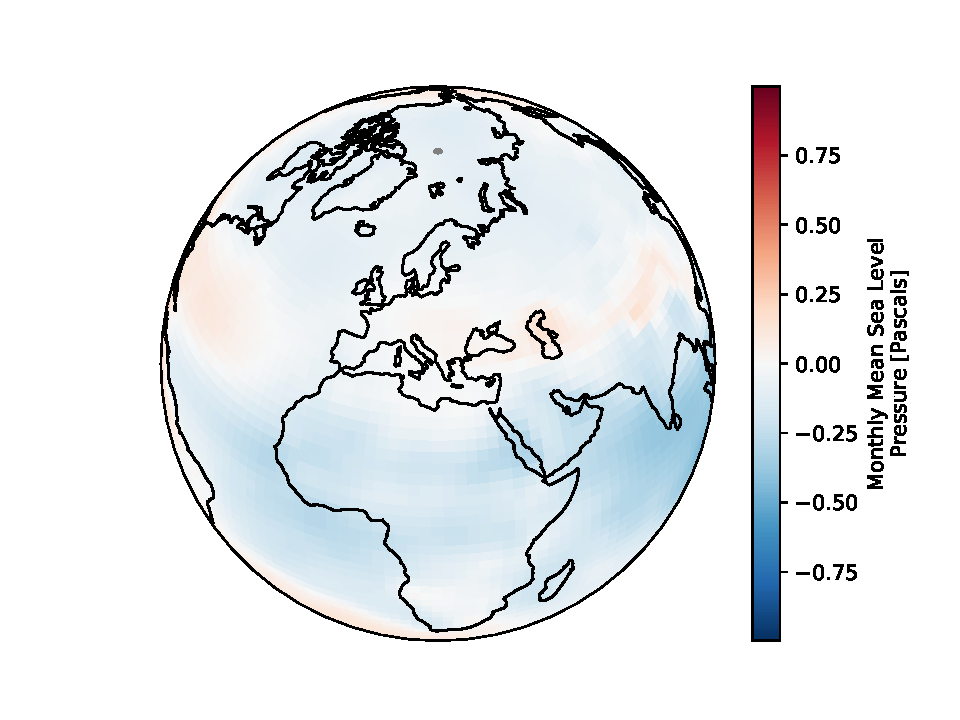
\includegraphics[width=0.4\textwidth]{tahiti-europe.pdf}
\end{figure}

\end{frame}

\begin{frame}{NOA - 2-means clustering}

\begin{figure}
    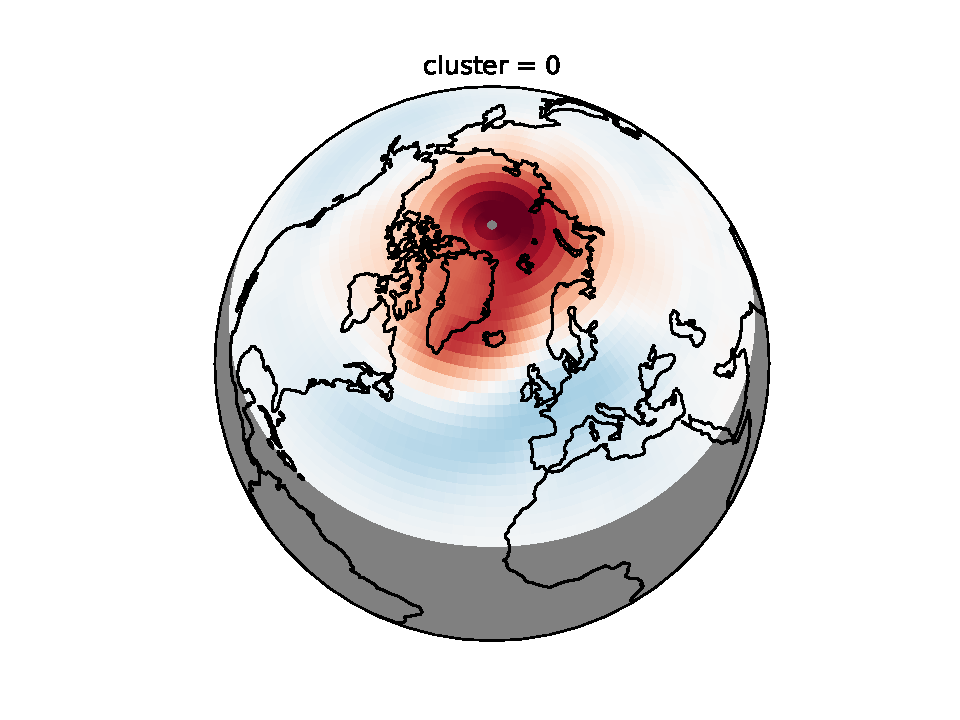
\includegraphics[width=0.4\textwidth]{nh-cluster0.pdf}%
    \hfill
    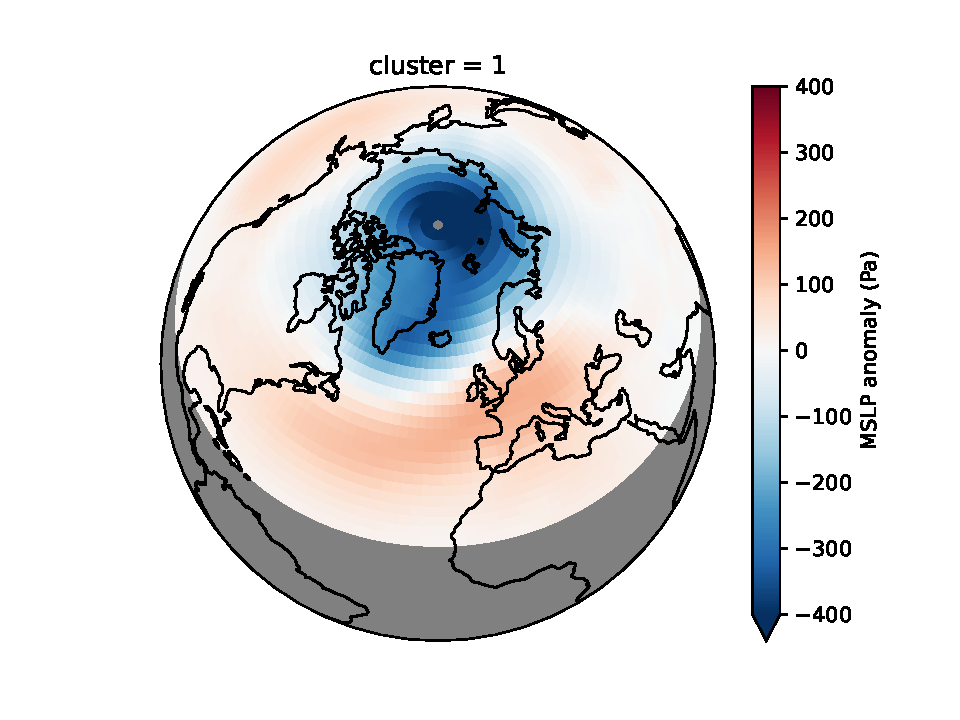
\includegraphics[width=0.4\textwidth]{nh-cluster1.pdf}
\end{figure}

\end{frame}







\end{document}
